\documentclass[11pt,a4paper]{article}
\author{TalentSprint}
\date{}
\usepackage{verbatim}
\usepackage{fancyhdr}           % For header and footer
\usepackage{multicol}
\usepackage{colortbl}           % For coloured tables
\usepackage{setspace}           % For line height
\usepackage{seqsplit}           % Splits long words.
\usepackage{amsmath} 
\usepackage{graphicx}
\usepackage{array}
\usepackage{enumitem}
\usepackage{xcolor}
\usepackage[tikz]{bclogo}
\usepackage{textcomp}
\usepackage{listings}
\lstset{language=python,numbers=left,numberstyle=\tiny,numbersep=10pt,showstringspaces=false}

\headheight=14pt
\lhead{\nouppercase{}}
\rhead{\nouppercase{\leftmark}}

\graphicspath{{../Images/} {../ScreenShots/}}
\setcounter{tocdepth}{1}
\setlength\parindent{0pt}
\parskip=4pt
\newcommand{\Code}[1]{\textbf{\texttt{#1}}}
%\thispagestyle{empty}
\begin{comment}
\def\AnswerBox{\fbox{\begin{minipage}{4in}\hfill\vspace{0.5in}\end{minipage}}}


\vspace{1.5pc}
\topskip0pt
\vspace*{\fill}
\centerline{\Huge Modern Programming}
\vspace{2pc}
\centerline{\Huge Practice}
\vspace{2pc}
\centerline{\Large using Python}
\vspace*{\fill}
\centerline{Prepared by TalentSprint WISE Team} 
\setcounter{page}{1}


\end{comment}
%========================================================================

% Lengths and widths
\addtolength{\textwidth}{5cm}
\addtolength{\hoffset}{-1cm}
\setlength{\headsep}{-12pt} % Reduce space between header and content
\setlength{\headheight}{85pt} % If less, LaTeX automatically increases it
\renewcommand{\footrulewidth}{2pt} % Remove footer line
\renewcommand{\headrulewidth}{1pt} % Remove header line
\renewcommand{\seqinsert}{\ifmmode\allowbreak\else\-\fi} % Hyphens in seqsplit
% This two commands together give roughly
% the right line height in the tables
\renewcommand{\arraystretch}{1.3}
\onehalfspacing



% Commands
\newcommand{\SetRowColor}[1]{\noalign{\gdef\RowColorName{#1}}\rowcolor{\RowColorName}} % Shortcut for row colour
\newcommand{\mymulticolumn}[3]{\multicolumn{#1}{>{\columncolor{white}}#2}{#3}} % For coloured multi-cols
\newcolumntype{x}[1]{>{\raggedright}p{#1}} % New column types for ragged-right paragraph columns
\newcommand{\tn}{\tabularnewline} % Required as custom column type in use

% Font and Colours
\definecolor{HeadBackground}{HTML}{333333}
\definecolor{FootBackground}{HTML}{666666}
\definecolor{TextColor}{HTML}{333333}
\definecolor{DarkBackground}{HTML}{6B8E23} %{FD1AA8}
\definecolor{LightBackground}{HTML}{E8FED8} %D3FDC8
\definecolor{tit}{HTML}{FF6600}
\renewcommand{\familydefault}{\sfdefault}
\color{TextColor}
 \headsep = 25pt
% Header and Footer
\pagestyle{fancy}
\usepackage[headheight=110pt]{geometry}
\fancyhf{}% Clear header/footer

\fancyhead[r]{
\includegraphics[width = 4cm, height = 2cm]{TS-Logo.png}\hspace{0cm}}

%=================================TITLE=====================================
\fancyhead[l]{\Large{\bf{\textcolor{tit}{\textrm{Functions}}}}}
%===========================================================================

\renewcommand{\headrulewidth}{0.4pt}% Default \headrulewidth is 0.4pt
\renewcommand{\footrulewidth}{0.4pt}% Default \footrulewidth is 0pt

\rfoot{Page \thepage}
\lfoot{COPYRIGHT \textcopyright TALENTSPRINT, 2015. ALL RIGHTS RESERVED.}




\begin{document}


%\chapter*{Functions}
A function is a block of organized, reusable code that is used to perform a single, related action.
Functions provide better modularity for your application and a high degree of code reusing.

As you already know, Python gives you many built-in functions like \emph{print()}, etc., but you can also create your own functions.
These functions are called \emph{user-defined functions}.

\section*{Defining a Funcion}

You can define functions to provide the required functionality. Here are simple rules to define a function in Python.
\begin{itemize}
\item Function blocks begin with the keyword \emph{def} followed by the function name and parentheses ().
\item Any input parameters or arguments should be placed within these parentheses. 
\item The code block within every function starts with a colon (:) and is indented.
\item The statement return [expression] exits a function, optionally passing back an expression to the caller. A return statement with no arguments is the same as return None.
\end{itemize}

\textbf{Syntax}
\begin{lstlisting}
def functionName():
    statement1
    statement2
    return [expression]
\end{lstlisting}

\section*{Calling a Function}
Defining a function only gives it a name, specifies the parameters that are to be included in the function and structures the blocks of code.

Once the basic structure of a function is finalized, you can execute it by calling it from another function or directly from the Python prompt.
\begin{verbatim}
>>> functionName()
\end{verbatim}

\begin{description}

\item[Example 1] print the sum of all even numbers in a given range.

\lstinputlisting{../Code/Program-11-1.py}

\item[Example 2] print all palindrome numbers, which contains all even digits.

\begin{figure}[ht]
\begin{center}
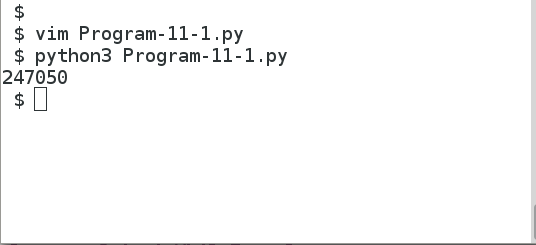
\includegraphics[scale=0.4]{Output-11-1.png}
\caption{Output}
\label{Output-11-1}
\end{center}
\end{figure}

\lstinputlisting{../Code/Program-11-2.py}

\begin{figure}[ht]
\begin{center}
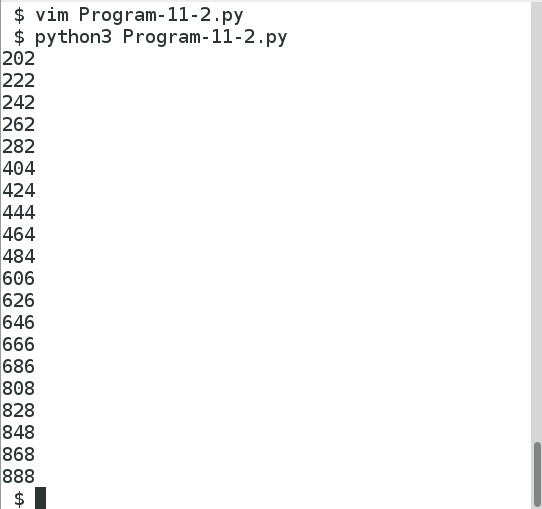
\includegraphics[scale=0.4]{Output-11-2.png}
\caption{Output}
\label{Output-11-2}
\end{center}
\end{figure}
\end{description}
\vfill{}
\section*{Returning Multiple Values}
A function can return exactly one value, or we should better say one object. An object can be a value of any type like., \emph{integer, float} or \emph{boolean} and it can also be a \emph{list} or a \emph{tuple}. So, if we have to return more than one value, we can use \emph{list} or \emph{tuple} for returning multiple values.

Example:

\begin{description} 
\item A program to print all two digit perfect square numbers.
\lstinputlisting{../Code/Program-11-3.py}
\begin{figure}[ht]
\begin{center}
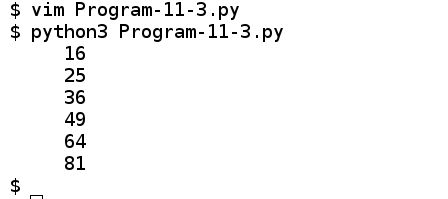
\includegraphics[scale=0.5]{Output-11-3.png}
\caption{Output}
\label{Output-11-3}
\end{center}
\end{figure}

\end{description}

\end{document}

